\documentclass[10pt, landscape]{article}
\usepackage[scaled=0.92]{helvet}
\usepackage{calc}
\usepackage{multicol}
\usepackage[a4paper,margin=3mm,landscape]{geometry}
\usepackage{amsmath,amsthm,amsfonts,amssymb}
\usepackage{color,graphicx,overpic}
\usepackage{dsfont}
\usepackage{hyperref}
\usepackage{newtxtext} 
\usepackage{enumitem}
\usepackage{esdiff}
\usepackage[table, dvipsnames]{xcolor}
\usepackage{mathtools}
\setlist{nosep}
\usepackage{tikz}
\usetikzlibrary{shapes.geometric}
\usepackage{makecell}  % for line break withih tabular
\usepackage{ulem}
\usepackage{calrsfs}
\normalem

% for including images
\graphicspath{ {./images/} }

\pdfinfo{
  /Title (st3248-midterm.pdf)
  /Creator (TeX)
  /Producer (pdfTeX 1.40.0)
  /Author (Yu Chenbo)
  /Subject (ST3248)
/Keywords (ST3248, nus, cheatsheet, pdf)}

% Turn off header and footer
\pagestyle{empty}

% redefine section commands to use less space
\makeatletter
\renewcommand{\section}{\@startsection{section}{1}{0mm}%
  {-1ex plus -.5ex minus -.2ex}%
  {0.5ex plus .2ex}%x
{\normalfont\large\bfseries}}
\renewcommand{\subsection}{\@startsection{subsection}{2}{0mm}%
  {-1explus -.5ex minus -.2ex}%
  {0.5ex plus .2ex}%
{\normalfont\normalsize\bfseries}}
\renewcommand{\subsubsection}{\@startsection{subsubsection}{3}{0mm}%
  {-1ex plus -.5ex minus -.2ex}%
  {-1ex plus .2ex}%
{\normalfont\small\bfseries\itshape}}%
\makeatother

\renewcommand{\familydefault}{\sfdefault}
\renewcommand\rmdefault{\sfdefault}
%  makes nested numbering (e.g. 1.1.1, 1.1.2, etc)
\renewcommand{\labelenumii}{\theenumii}
\renewcommand{\theenumii}{\theenumi.\arabic{enumii}.}
\renewcommand\labelitemii{•}
\renewcommand\labelitemiii{•}

\definecolor{mathblue}{cmyk}{1,.72,0,.38}
\everymath\expandafter{\the\everymath \color{mathblue} }

% Don't print section numbers
\setcounter{secnumdepth}{0}

\setlength{\parindent}{0pt}
\setlength{\parskip}{0pt plus 0.5ex}
%% this changes all items (enumerate and itemize)
\setlength{\leftmargini}{0.5cm}
\setlength{\leftmarginii}{0.5cm}
\setlist[itemize,1]{leftmargin=2mm,labelindent=1mm,labelsep=1mm}
\setlist[itemize,2]{leftmargin=2mm,labelindent=1mm,labelsep=1mm}
\setlist[itemize,3]{leftmargin=2mm,labelindent=1mm,labelsep=1mm}

% adding my commands
\input{../Latex/Util/style-helpers.tex}
\input{../Latex/Util/code.tex}
\input{../Latex/Util/math.tex}
\input{../Latex/Util/joins.tex}

% aliasing commands
\newcommand{\eps}{\varepsilon}
% \newcommand{\ta}{\textbf{a}}
% \newcommand{\tb}{\textbf{b}}
% \newcommand{\tc}{\textbf{c}}
% \newcommand{\tr}{\textbf{r}}

\DeclareMathOperator*{\argmax}{arg\,max}
\DeclareMathOperator*{\argmin}{arg\,min}

% -----------------------------------------------------------------------

\begin{document}
\raggedright
\begin{multicols*}{3}
    \section{Statistical Learning}
    \begin{itemize}
      \item \uline{\textbf{Prediction:}} predict $Y$ using $\hat{f}(X)$, where the exact form of $\hat{f}$ is not cared about.
      \item $E(Y - \hat{Y})^2 = E[f(X) + \eps - \hat{f}(X)] ^ 2 = \underbrace{[f(x) - \hat{f}(X)]^2}_\text{reducible} + \underbrace{Var(\eps)}_\text{irreducible}$
      \item \uline{\textbf{Inference:}} explore how $Y$ changes as a function of predictors $X_i$, not necessarily to make predictions.
      \item How to estimate f?
      \begin{itemize}
        \item \textbf{Parametric approach}: hypothesise a model and try to fit the parameters.
        \item \textbf{Non-parametric approach:} try to find a $\hat{f}$ that's close to the data points, requiring a large number of observations.
        \item Flexibility of a model is a trade-off between accuracy and interpretability when \uline{not overfitting}.
      \end{itemize}
      \item \uline{\textbf{Bias-variance trade-off:}}
      \begin{itemize}
        \item Expected test MSE = $E[y_0 - \hat{f}(x_0)]^2 = Var(\hat{f}(x_0)) + [Bias(\hat{f}(x_0))]^2 + Var(\eps)$
        \item When flexibility increases, bias initially decreases faster than the variance increases. Test MSE decreases.
        \item After reaching the point where bias stops decreasing very much anymore, test MSE increases.
      \end{itemize}
      \item \uline{\textbf{Classification:}}
      \begin{itemize}
        \item Bayes Classifier: $\hat{y_0} = \mathrm{argmax}_j P(Y = j|X = x_0)$
        \item Bayes Error Rate: $1 - E[\max_j P(Y=j|X)]$
        \item Bayes error rate $>$ 0 iff classes overlap (irreducible error).
      \end{itemize}
      \item KNN: $\hat{P}(Y=j|X=x_0)={1\over K} \sum_{i\in \mathcal{N}_0} \mathds{1}(y_i = j)$
      \item Small K: low bias. Big K: low variance.
    \end{itemize}

    \section{Linear Regression}
    \subsection{Simple Linear Regression}
    \begin{itemize}
      \item Model: $\hat{y_i} = \hat{\beta_0} + \hat{\beta_1}x_i $
      \item OLS estimates: $\hat{\beta_0} = \bar{y} - \hat{\beta_1}\bar{x}$, $\hat{\beta_1} = \frac{\sum_{i=1}^n (x_i - \bar{x})(y_i - \bar{y})}{\sum_{i=1}^n (x_i - \bar{x})^2}$
      \item The population regression line is $Y = \beta_0 + \beta_1X$ (true parameters).
      \item The least squares line is $\hat{Y} = \hat{\beta_0} + \hat{\beta_1}X$ (estimated parameters, changes with different training data).
      \item $\hat{\beta_0}$ and $\hat{\beta_1}$ are unbiased estimators of $\beta_0$ and $\beta_1$.
      \item $SE(\hat{\beta_0})^2 = \sigma^2 \left[ \frac{1}{n} + \frac{\bar{x}^2}{\sum_{i=1}^n (x_i - \bar{x})^2} \right]$, $SE(\hat{\beta_1})^2 = \frac{\sigma^2}{\sum_{i=1}^n (x_i - \bar{x})^2}$, where $\sigma^2 = \text{Var}(\eps)$.
      \item In practice, $\sigma^2$ is unknown and is estimated by $\text{RSE}^2 = \frac{1}{n-2} \sum_{i=1}^n (y_i - \hat{y_i})^2$.
      \item Approximate 95\% confidence interval for $\beta_j$ is $\hat{\beta_j} \pm 2 \times SE(\hat{\beta_j})$.
      \item t-test: for $H_0: \beta_j = 0$ and $H_1: \beta_j \neq 0$, calculate $t = \frac{\hat{\beta_j} - 0}{SE(\hat{\beta_j})}$, where $t \sim t_{n-2}$.
      \item \textbf{Accessing model accuracy:}
      \begin{itemize}
        \item RSE measures the lack of fit of the model to the data.
        \item {R-squared:} proportion of variance explained by the model. $R^2 = \frac{TSS - RSS}{TSS} = 1 - \frac{RSS}{TSS}$, where $TSS = \sum_{i=1}^n (y_i - \bar{y})^2$ and $RSS = \sum_{i=1}^n (y_i - \hat{y_i})^2$.
        \item For simple linear regression, $R^2 = r^2$, where $r = \hat{\text{Cor}}(X,Y) = \frac{\sum_{i=1}^n (x_i - \bar{x})(y_i - \bar{y})}{\sqrt{\sum_{i=1}^n (x_i - \bar{x})^2 \sum_{i=1}^n (y_i - \bar{y})^2}}$.
      \end{itemize}
    \end{itemize}

    \subsection{Multiple Linear Regression}
    \begin{itemize}
      \item Model: $\hat{y_i} = \hat{\beta_0} + \hat{\beta_1}x_{i1} + \hat{\beta_2}x_{i2} + \ldots + \hat{\beta_p}x_{ip}$
      \item $\beta_i$ is the average effect on $Y$ of one unit increase in $X_i$, \textbf{holding all other predictors fixed}.
      \item \textbf{F-test:} 
      \begin{itemize}
        \item $H_0: \beta_1 = \beta_2 = \ldots = \beta_p = 0$ and $H_1: \text{at least one} \neq 0$, calculate $F = \frac{(TSS - RSS)/p}{RSS/(n-p-1)}$, where $F \sim F_{p, n-p-1}$.
        \item Under $H_0$, F is around 1. Under $H_1$, F is greater than 1.
        \item Even if $H_0$ is true, individual p-values for t-test can be significant due to inflation of Type I error in multiple testing.
      \end{itemize}
      \item \textbf{Model selection:}
      \begin{itemize}
        \item benchmark: RSS
        \item stopping rule: p-value
        \item forward, backward selection: $1+\frac{p(p+1)}{2}$ models, mixed selection
      \end{itemize}
      \item \textbf{Model accuracy:} $RSE = \sqrt{\frac{1}{n-p-1} RSS}$, $R^2$ and graph (to investigate synergy).
      \item \textbf{Prediction interval} accounts for both the \uline{reducible} and \uline{irreducible error}, hence targets individual observations.
      \item \textbf{Confidence interval} only accounts for the \uline{reducible error}, hence targets the average and is narrower.
    \end{itemize}

    \subsection{Other Considerations}
    \begin{itemize}
      \item For predictors with $k\ge2$ levels: use $k-1$ dummy variables.
      \item \textbf{Interaction term} coefficient interpretation: the increase in the effectiveness of A for a one-unit increase in B.
      \item If the interaction term is significant, the main effects should be kept in the model.
      \item \textbf{Interaction term} of a qualitative with a quantitative variable gives different slopes for different levels of the qualitative variable.
      \item \textbf{Non-linear relationships:} polynomial regression.
    \end{itemize}

    \subsection{Problems and Solutions}
    \begin{itemize}
      \item Non-linearity: identify using residual plots (e against x/y), add powers of x, log(x), $\sqrt{x}$, etc.
      \item Correlation in $\eps$: makes SEs, CIs and PIs \textbf{underestimated}. Identify with residual plots.
      \item Non-constant variance (heteroscedasticity): identify with residual plots, transform with $\sqrt{Y}$, $\log{Y}$, etc. When the variance follows a function, use weighted least squares with weights inversely proportional to the variance.
      \item Outliers: identify with studentized residuals (typically $>3$).
      \item High leverage points: calculate $h_i = \frac{1}{n} + \frac{(x_i - \bar{x})^2}{\sum_{j=1}^n (x_j - \bar{x})^2}$. Average leverage is $\frac{p+1}{n}$.
      \item Collinearity: $\hat{\beta}$ for correlated predictors have high variance, hence large SEs and p-values. $VIF(\hat{\beta_j}) = \frac{1}{1 - R^2_{X_j|X_{-j}}}$, where $R^2_{X_j|X_{-j}}$ is the $R^2$ of $X_j$ regressed on all other predictors. VIF $> 5$ is a sign of collinearity.
    \end{itemize}

    \subsection{KNN Regression}
    \begin{itemize}
      \item $\hat{f}(x_0)={1\over K} \sum_{i\in \mathcal{N}_0} y_i$.
      \item When p = 1, KNN is much better than OLS for non-linear relationships.
      \item For higher ps, KNN is not as good as OLS: curse of dimensionality.
    \end{itemize}

    \section{Classification}
    \subsection{Logistic Regression}
    \begin{itemize}
      \item $p(X) = P(Y=1|X) = \frac{e^{\beta_0 + \beta_1X}}{1 + e^{\beta_0 + \beta_1X}}$
      \item logit: $\log \left( \frac{p(X)}{1 - p(X)} \right) = \beta_0 + \beta_1X$
      \item $L(\beta_0, \beta_1) = \prod_{i:y_i=1} p(x_i) \prod_{i:y_i=0} (1 - p(x_i))$
    \end{itemize}

    \subsection{Linear Discriminant Analysis}
    \begin{itemize}
      \item $\pi_k = P(Y=k)$, $f_k(X) = P(X=x|Y=k)$
      \item $p_k(x) = P(Y=k|x) = \frac{\pi_k f_k(x)}{\sum_{l=1}^K \pi_l f_l(x)}$, posterier probability.
      \item Assume $f_k(x) = \frac{1}{\sqrt{2\pi} \sigma_k} \text{exp}(-\frac{1}{2\sigma_k^2} (x - \mu_k)^2)$, and $\sigma_k = \sigma$. $p_k(x) = \frac{\pi_k \text{exp}(-\frac{1}{2\sigma^2} (x - \mu_k)^2)}{\sum_{l=1}^K \pi_l \text{exp}(-\frac{1}{2\sigma^2} (x - \mu_l)^2)}$.
      \item $\delta_k(x) = x \frac{\mu_k}{\sigma^2} - \frac{\mu_k^2}{2\sigma^2} + \log(\pi_k)$
      \item Estimates: $\hat{\pi_k} = \frac{n_k}{n}$, $\hat{\mu_k} = \frac{1}{n_k} \sum_{i:y_i=k} x_i$, $\hat{\sigma}^2 = \frac{1}{n-K} \sum_{k=1}^K \sum_{i:y_i=k} (x_i - \hat{\mu_k})^2$
      \item For $p>1$, $\delta_k(x) = x^T \Sigma^{-1} \mu_k - \frac{1}{2} \mu_k^T \Sigma^{-1} \mu_k + \log(\pi_k)$, where $\Sigma$ is the covariance matrix.
      \item \textbf{Sensitivity}: true positive rate, \textbf{specificity}: true negative rate. Nudge the softmax threshold to adjust sensitivity and specificity.
      \item ROC curve: plot sensitivity against 1 - specificity.
    \end{itemize}

    \subsection{Quadratic Discriminant Analysis}
    {\small
    \begin{align*}
      \delta_k(x) &= -\frac{1}{2} \log |\Sigma_k| - \frac{1}{2} (x - \mu_k)^T \Sigma_k^{-1} (x - \mu_k) + \log(\pi_k) \\ 
      &= -\frac{1}{2} x^T \Sigma_k^{-1} x + x^T \Sigma_k^{-1} \mu_k - \frac{1}{2} \mu_k^T \Sigma_k^{-1} \mu_k - \frac{1}{2} \log |\Sigma_k| + \log(\pi_k)
    \end{align*}
    }
    \begin{itemize}
      \item $p(p+1)/2$ parameters for $\Sigma_k$.
    \end{itemize}
    
    \section{Resampling Methods}
    \begin{itemize}
      \item Validation set: variable MSE, tends to overestimate test error rate.
      \item LOOCV: far less bias but costly. \textbf{For least squares}, $\text{CV}_{(n)} = \frac{1}{n} \sum_{i=1}^n \left( \frac{y_i - \hat{y_i}}{1 - h_i} \right)^2$, where $h_i$ is the leverage.
      \item LOOCV vs. k-fold CV: highly positively correlated MSEs result in higher variance. More pronounced for big p and small n.
      \item Bootstrap:
      \begin{itemize}
        \item Minimise $\text{Var}(\alpha X + (1-\alpha) Y)$: $\alpha = \frac{\sigma^2_Y-\sigma_{XY}}{\sigma^2_X + \sigma^2_Y - 2\sigma_{XY}}$
        \item Bootstrap resampling: sample with replacement n observations, repeat B times.
        \item If bootstrap SE estimates for regression models differ from the analytical SE estimates, the model is not a good fit.
      \end{itemize}
    \end{itemize}

    \section{Linear Model Selection and Regularization}
    \subsection{Subset Selection}
    \subsubsection{Best subset selection}
    \begin{itemize}
      \item Use RSS to compare among models with the same k, then CV to compare across the p + 1 models. $2^p$ models.
    \end{itemize}
    \subsubsection{Stepwise selection}
    \begin{itemize}
      \item Reduce the search space because of computational limitations and avoid finding "too good" models that overfit.
      \item In each step, extends the model by adding or removing one predictor with the smallest RSS or largest $R^2$.
      \item Among the p + 1 models obtained, choose using CV, $C_p$, AIC, BIC, adjusted $R^2$.
      \item $1+p(p+1)/2$ models. However, when $n<p$, only have $\mathcal{M}_0$ up to $\mathcal{M}_{n-1}$.
    \end{itemize}
    \subsubsection{Model selection criteria}
    \begin{itemize}
      \item $C_p = \frac{1}{n} (RSS + 2d\hat{\sigma}^2)$, where $d$ is the number of predictors and $\hat{\sigma}^2$ is the estimated $\text{Var}(\eps)$.
        Typically, $\hat{\sigma}^2$ is estimated using the full model. Theory: $C_p$ is an unbiased estimate of test MSE if $\hat{\sigma}^2$ is unbiased.
      \item $\text{AIC} = \frac{1}{n\hat{\sigma}^2} (RSS + 2d\hat{\sigma}^2)$.
      \item $\text{BIC} = \frac{1}{n\hat{\sigma}^2} (RSS + \log(n)d\hat{\sigma}^2)$, heavier penalty on d.
      \item Adjusted $R^2 = 1 - \frac{RSS/(n-d-1)}{TSS/(n-1)}$.
      \item CV methods make fewer assumptions about the true model. Better when hard to: find effective number of predictors, estimate $\hat{\sigma}^2$ or when asymptotics are not realistic, e.g. n not much bigger than p.
    \end{itemize}

    \subsection{Shrinkage Methods}
    \subsubsection{Ridge Regression}
    \begin{itemize}
      \item Target: $\sum_{i=1}^n (y_i - \beta_0 - \sum_{j=1}^p \beta_j x_{ij})^2 + \lambda \sum_{j=1}^p \beta_j^2$.
      \item $X_j\hat{\beta}^{R}_{j,\lambda}$ depends on both $\lambda$ and the scaling of $X$, unlike in OLS where $X_j\hat{\beta}_j$ is constant.
      \item Hence, standardisation is necessary to make $X_i$ have mean 0 and sd 1.
      \item Ridge regression trades off a small increase in bias for a large decrease in variance. It works well for $p \approx n$ and $p > n$.
      \item 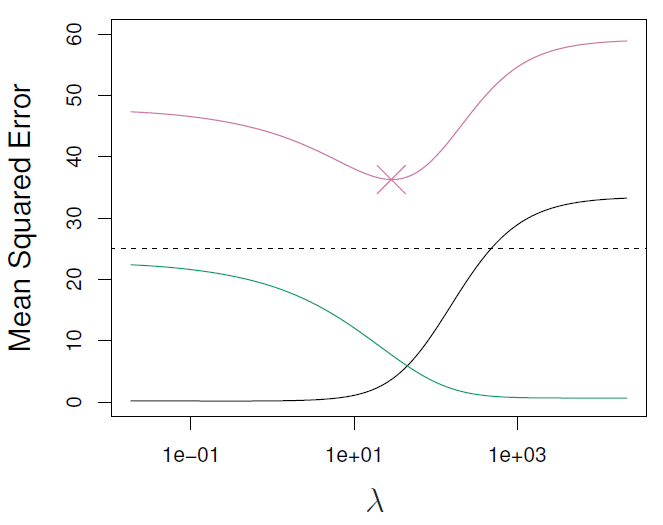
\includegraphics[width=0.9\linewidth]{st3248-final-ridge.png}
    \end{itemize}
    \subsubsection{Lasso}
    \begin{itemize}
      \item Target: $\sum_{i=1}^n (y_i - \beta_0 - \sum_{j=1}^p \beta_j x_{ij})^2 + \lambda \sum_{j=1}^p |\beta_j|$.
      \item Optimisation dual: $\argmin_{\beta} \text{RSS} \text{ s.t. } \sum_{j=1}^p |\beta_j| \le s$.
      \item Best subset selection: $\sum_{j=1}^p \mathds{1}(\beta_j \neq 0) \le s$.
      \item Ridge performs better when all coeffs are of roughly equal size.
    \end{itemize}

    \subsection{Dimension Reduction Methods}
    \begin{itemize}
      \item Let $Z_m = \sum_{j=1}^p \phi_{jm}X_j$, for $m=1,2,\ldots,M$. This constrains $\hat{\beta}_j$ to be linear combinations.
      \item This increases the bias, but reduces the variance if p is large and M$<<$p.
      \item If M=p and $Z_m$ are orthogonal, no change.
    \end{itemize}
    \subsubsection{Principal Components Regression}
    \begin{itemize}
      \item First principle component: $Z_1 = \phi_{11}(X_1 - \bar{X_1}) + \phi_{21}(X_2 - \bar{X_2}) + \ldots + \phi_{p1}(X_p - \bar{X_p})$, where $\text{Var}(Z_1)$ is maximised subject to $\sum_{j=1}^p \phi_{j1}^2 = 1$.
      \item Assumption: the directions of $Z_i$s are associated with the response.
      \item Ridge regression is closely related to PCR.
      \item Favours bigger scale predictors, hence need to standardise.
    \end{itemize}
    \subsubsection{Partial Least Squares}
    \begin{itemize}
      \item First PLS direction: Standardise all $X_i$s. $\phi_{j1} =$ coefficient of $\text{SLR}(Y\sim X_j)$
      \item Second: For $k = 1,\ldots,p$, run $\text{SLR}(X_k \sim Z_1)$ to obtain $e_k^{(1)}$ used as $X_k^{(1)}$.
    \end{itemize}
    \columnbreak
    \subsubsection{High Dimensional Problems}
    \begin{itemize}
      \item When p is large, the multicolllinearity problem is severe. The set of signal predictors obtained from one dataset may not be the true predictors.
      \item Test error on an independent test set or CV errors are the only good measures.
    \end{itemize}

    \section{Unsupervised Learning}
    \subsection{PCA}
    \begin{itemize}
      \item Computation: Center $\bf{X}$. Solve $\max{\frac{1}{n}\sum_{i=1}^n \left( \sum_{j=1}^p \phi_{j1}x_{ij} \right)^2}$ subject to $\sum_{j=1}^p \phi_{j1}^2 = 1$.
      \item Alternative interpretation: low-dimensional linear sufaces that are closest to the observations.
      \item When $M = \min(n-1, p)$, the surface is exact.
      \item Need to standardise.
      \item Proportion of variance explained (PVE) of the {\itshape{m}}th principle component: $\frac{\sum_{i=1}^n \left( \sum_{j=1}^p \phi_{jm}x_{ij} \right)^2}{\sum_{i=1}^n \sum_{j=1}^p x_{ij}^2}$.
    \end{itemize}

    \subsection{Clustering}
    \subsubsection{K-means}
    \begin{itemize}
      \item Minimise pairwise squared Euclidean distance: $\frac{1}{|C_k|}\sum_{i,i' \in C_k} \sum_{j=1}^p (x_{ij} - x_{i'j})^2$.
      \item Local minimum algorithm: 1. Randomly assign clusters. 2. Compute centroids. 3. Assign each observation to the closest centroid.  
    \end{itemize}
    \subsubsection{Hierarchical Clustering}
    \begin{itemize}
      \item Caveat: The true structure may not be nested. (e.g. gender and nationality)
      \item Linkage: complete (max pairwise dissimilarity), single (min), average (mean), centroid (between centroids).
      \item Average and complete preferred, single leads to one-at-a-time fusion.
      \item Correlation-based distance: focuses on the shapes of the observations rather than the magnitudes.
      \item Standardisation may be necessary.
    \end{itemize}
    \subsubsection{Remarks}
    \begin{itemize}
      \item Outliers or perturbations can have a big impact.
    \end{itemize}


    \section{R}
    \begin{itemize}
      \item lm() summary reports t-statistics and p-values for each predictor, \textbf{after adjusting for other predictors}.
      \item hatvalues() returns the leverage of each observation.
      \item anova() compares models.
      \item glmnet() alpha = 0 for ridge, alpha = 1 for lasso.
      \item pcr() $\text{CV} = \sqrt{\text{MSE}}$
      \item square sdev and divide by total var to get PVE.
    \end{itemize}
\end{multicols*}
\end{document}